\documentclass[letterpaper,12pt]{article}
% \usepackage[utf8]{inputenc}
\usepackage{cinvestav_style}
% \usepackage[demo]{graphicx}
\usepackage{subcaption}

%opening
\title{}
\author{Isaac Ayala Lozano}
\date{}

\begin{document}

% \maketitle

\section{Movimiento de una part\'icula en $\mathbb{R}^3$}

 \subsection{Ecuaciones de movimiento}
 
 Se definen de la siguiente manera: $ x(t) = 0$, $y (t) = 0 $, $z (t) = z_0 + v_0 t - \frac{1}{2} g t^2$.

 \section{Simulaci\'on}
 
 Se evalu\'o el sistema con las condiciones iniciales $z_0 = 0$ y $v_0 = 0$. La figura \ref{fig: free fall - 0} presenta las gr\'aficas de $z(t)$ en los planos \emph{tz} y \emph{xz}. Es importante observar que la gr\'afica en el plano \emph{xz} es id\'entica a la gr\'afica en el plano \emph{yz} debido a que las coordenadas \emph{x} y \emph{y} preservan su valor inicial 0.
 
 \begin{figure}[h]
\begin{subfigure}{.5\textwidth}
  \centering
  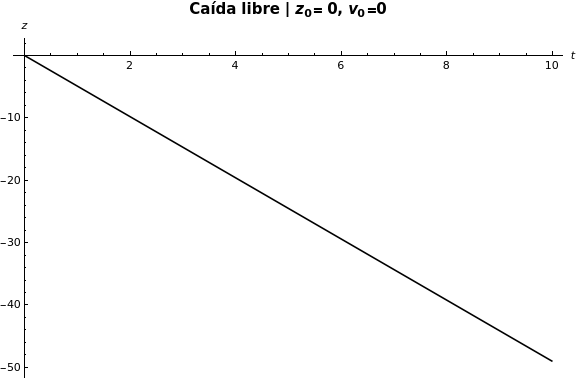
\includegraphics[width=.8\linewidth]{freefallgraph.png}
  \caption{Plano tz.}
  \label{fig: tz plane}
\end{subfigure}%
\begin{subfigure}{.5\textwidth}
  \centering
  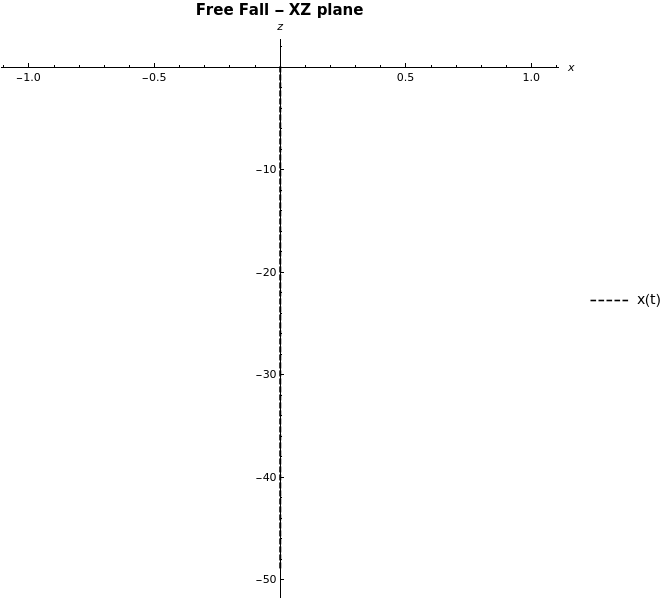
\includegraphics[width=.8\linewidth]{freefallgraphxz.png}
  \caption{Plano xz.}
  \label{fig: xz plane}
\end{subfigure}
\caption{Ca\'ida libre - condiciones iniciales 0}
\label{fig: free fall - 0}
\end{figure}
 
 
 El sistema fue probado tambi\'en con condiciones iniciales $z_0 \in \{1, 10, 100, 100\}$ y $v_0 \in \{1, 10, 100, 100\}$. La figura \ref{fig: free fall - initial condition matrix} presenta las gr\'aficas de $z(t)$ en el plano \emph{tz} para distintas combinaciones de las condiciones iniciales.
 
 
  \begin{figure}[h]
\begin{subfigure}{\textwidth}
  \centering
  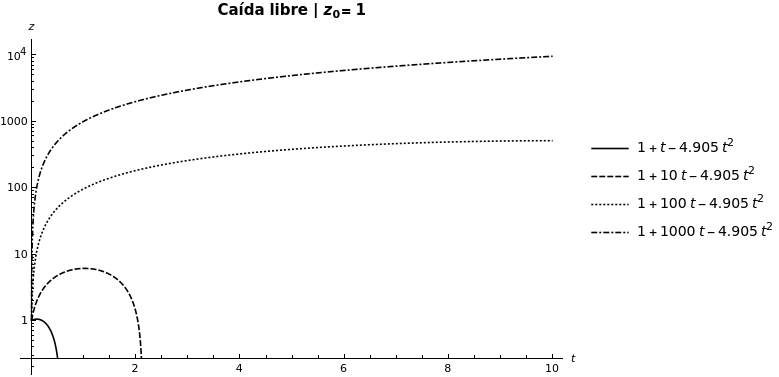
\includegraphics[scale=0.4]{loggraph01.png}
  \caption{Condici\'on $z_0=0$.}
  \label{fig: a}
\end{subfigure}%
\\
\begin{subfigure}{\textwidth}
  \centering
  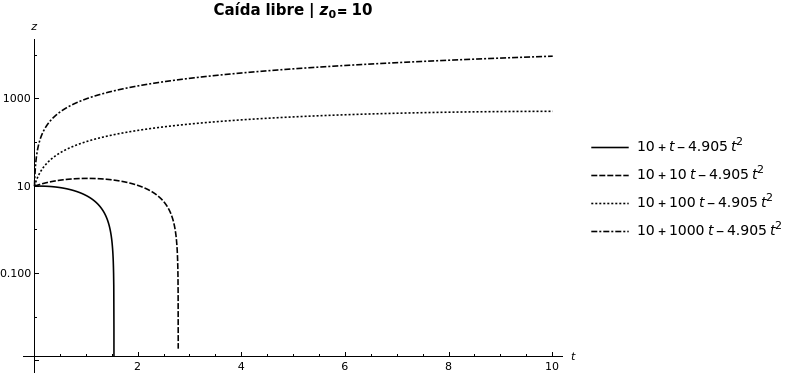
\includegraphics[scale=0.4]{loggraph02.png}
  \caption{Condici\'on $z_0=10$.}
  \label{fig: b}
\end{subfigure}
\begin{subfigure}{\textwidth}
  \centering
  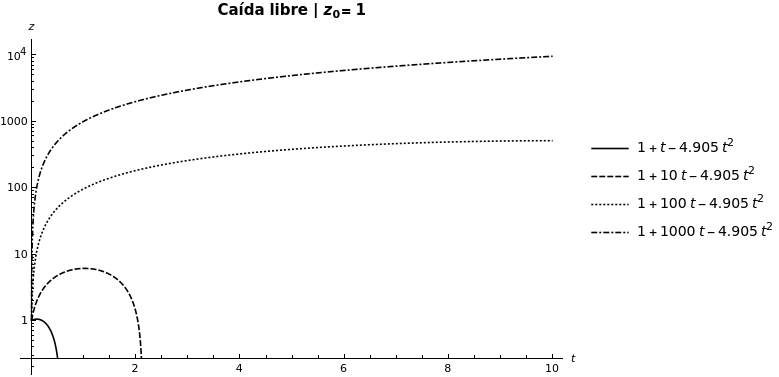
\includegraphics[scale=0.4]{loggraph01.png}
  \caption{Condici\'on $z_0=100$.}
  \label{fig: c}
\end{subfigure}%
\caption{Ca\'ida libre - alteraci\'on de condiciones iniciales.}
\label{fig: free fall - initial condition matrix}
\end{figure}
 
Observamos que la part\'icula eventualmente descender\'a y habr\'a un impacto con el piso en caso de existir, sin importar el valor inicial de su posici\'on. La condici\'on inicial de velocidad juega un papel mucho m\'as importante ya que \'este determina el comportamiento de la part\'icula. Observamos que para valores de $v_0$ con orden de magnitud 2 o mayor, el efecto de la aceleraci\'on disminuye considerablemente comparado con las otras condiciones iniciales.
\end{document}
